\documentclass[10pt]{article}
\usepackage[polish]{babel}
\usepackage[utf8]{inputenc}
\usepackage[T1]{fontenc}
\usepackage{amsmath}
\usepackage{amsfonts}
\usepackage{amssymb}
\usepackage[version=4]{mhchem}
\usepackage{stmaryrd}
\usepackage{graphicx}
\usepackage[export]{adjustbox}
\graphicspath{ {./images/} }

\begin{document}
\begin{enumerate}
  \item Liczby rzeczywiste \(a, b, c\) mają tę własność, że liczby \(a+b, a+c, b+c\) są trzema kolejnymi liczbami całkowitymi, \(z\) których największa jest nieparzysta. Udowodnij, że liczby \(a, b, c\) też są kolejnymi liczbami całkowitymi.
  \item Znajdź wszystkie pary ( \(m, n\) ) liczb całkowitych dodatnich, które spełniają równanie: \(4^{n}+260=m^{2}\)
  \item W trójkącie \(A B C\) punkty \(D, E, F\) są środkami boków, a punkt \(H\) spodkiem wysokości opuszczonej z wierzchołka A. Wykaż, że na czworokącie DEFH można opisać okrąg.\\
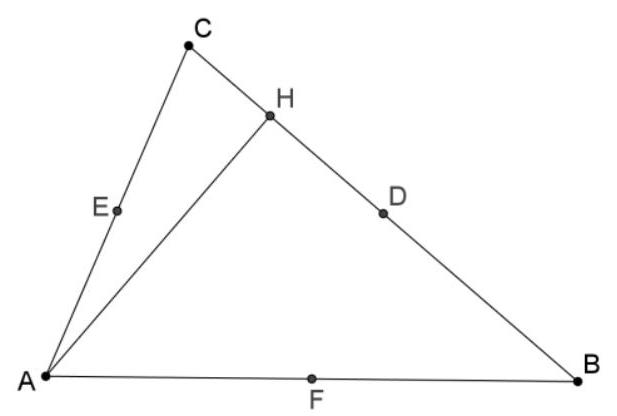
\includegraphics[max width=\textwidth, center]{2024_11_21_c9275076f143e55033f1g-1}
\end{enumerate}

\end{document}